\documentclass{article}
\usepackage[margin=1cm]{geometry}
\def\pgfsysdriver{pgfsys-dvisvgm.def}
\usepackage{pgfplots}
\pgfplotsset{compat=1.18}
\pagestyle{empty}
\begin{document}
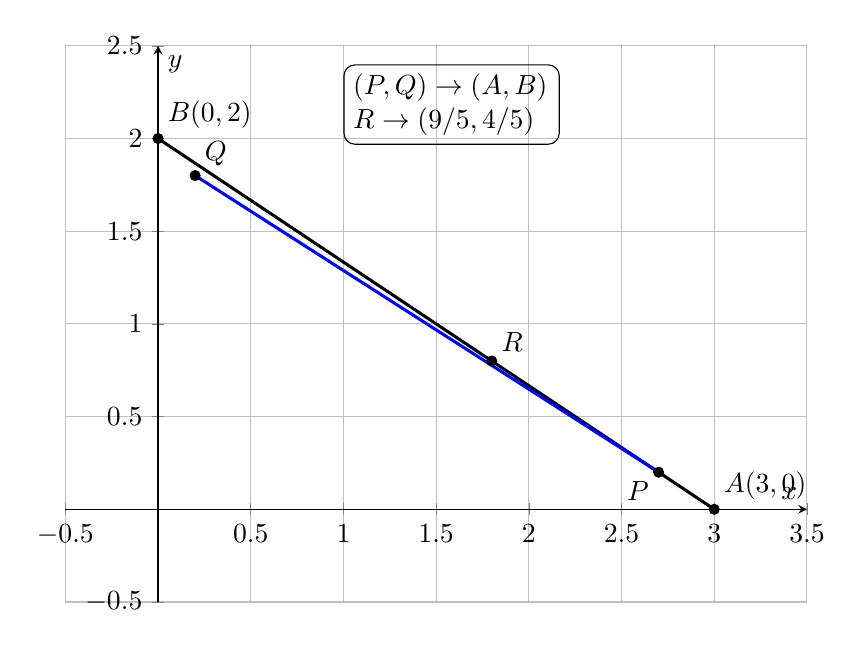
\begin{tikzpicture}
\begin{axis}[width=11cm,height=9cm,axis equal image,axis lines=middle,grid=major,xmin=-0.5,xmax=3.5,ymin=-0.5,ymax=2.5,xlabel={$x$},ylabel={$y$},clip=true]
  \addplot[black,line width=1.1pt] coordinates {(3,0) (0,2)};
  \addplot[blue,line width=1.1pt] coordinates {(2.7,0.2) (0.2,1.8)};
  \addplot[only marks,mark=*,mark size=1.8pt,black] coordinates {(3,0) (0,2) (2.7,0.2) (0.2,1.8) (1.8,0.8)};
  \node[anchor=south west] at (axis cs:3,0) {$A(3,0)$};
  \node[anchor=south west] at (axis cs:0,2) {$B(0,2)$};
  \node[anchor=north east] at (axis cs:2.7,0.2) {$P$};
  \node[anchor=south west] at (axis cs:0.2,1.8) {$Q$};
  \node[anchor=south west] at (axis cs:1.8,0.8) {$R$};
  \node[draw,rounded corners,align=left,anchor=north west,text width=2.5cm] at (axis cs:1.0,2.4) {$(P,Q)\to(A,B)$\\$R\to(9/5,4/5)$};
\end{axis}
\end{tikzpicture}
\end{document}
